\documentclass[tikz,border=3pt]{standalone}
\usepackage[utf8]{inputenc}
\usepackage[T1]{fontenc}
\usepackage{lmodern}
\renewcommand{\familydefault}{\sfdefault}
\usepackage{sansmath}\sansmath
\usepackage{chemfig}
\usepackage{pgfplots}\pgfplotsset{compat=1.18,/pgf/number format/use comma,/pgf/number format/1000 sep={.}}
\usetikzlibrary{arrows.meta,calc,positioning,decorations.pathmorphing,patterns}
% paleta del sitio
\definecolor{nar}{HTML}{E8680C}\definecolor{narc}{HTML}{FFB35C}\definecolor{hielo}{HTML}{FFF3E8}
\definecolor{tinta}{HTML}{1D1D1F}\definecolor{gris}{HTML}{6E6E73}\definecolor{lila}{HTML}{7C5CF0}
\definecolor{azul}{HTML}{2F6FD6}\definecolor{menta}{HTML}{17A673}\definecolor{coral}{HTML}{E8342A}
\begin{document}
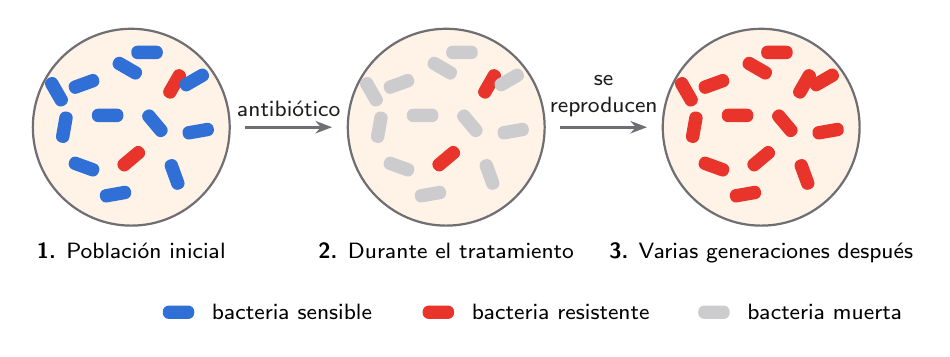
\begin{tikzpicture}[font=\small]
\tikzset{bac/.style={rounded corners=2.2pt,minimum width=0.4cm,minimum height=0.17cm,inner sep=0pt},
  flecha/.style={-{Stealth[length=6pt]},gris,very thick}}
\newcommand{\placa}[1]{\fill[hielo,draw=gris,thick] (#1,0) circle (1.25);}
% posiciones: x/y/giro
\def\pos{-0.6/0.55/20,-0.05/0.75/-30,0.55/0.55/60,-0.85/0/80,-0.3/0.15/0,0.3/0.05/-50,0.85/-0.05/10,-0.6/-0.5/-20,0/-0.4/40,0.55/-0.6/-70,-0.2/-0.85/10,0.2/0.95/0,-0.95/0.45/-60,0.8/0.6/30}
% 1: poblacion inicial (dos resistentes: indices 3 y 9)
\placa{0}
\foreach \x/\y/\g [count=\i] in \pos {\ifnum\i=3 \def\c{coral}\else\ifnum\i=9 \def\c{coral}\else\def\c{azul}\fi\fi
  \node[bac,fill=\c,rotate=\g] at (\x,\y) {};}
% 2: con antibiotico
\placa{4}
\foreach \x/\y/\g [count=\i] in \pos {\ifnum\i=3 \def\c{coral}\else\ifnum\i=9 \def\c{coral}\else\def\c{gris!35}\fi\fi
  \node[bac,fill=\c,rotate=\g] at (\x+4,\y) {};}
% 3: generaciones despues
\placa{8}
\foreach \x/\y/\g [count=\i] in \pos {\node[bac,fill=coral,rotate=\g] at (\x+8,\y) {};}
\draw[flecha] (1.45,0) -- (2.55,0) node[midway,above,font=\footnotesize,text=tinta] {antibiótico};
\draw[flecha] (5.45,0) -- (6.55,0) node[midway,above,font=\footnotesize,text=tinta,align=center] {se\\reproducen};
\node[anchor=north,align=center,font=\footnotesize] at (0,-1.35) {\textbf{1.} Población inicial};
\node[anchor=north,align=center,font=\footnotesize] at (4,-1.35) {\textbf{2.} Durante el tratamiento};
\node[anchor=north,align=center,font=\footnotesize] at (8,-1.35) {\textbf{3.} Varias generaciones después};
\begin{scope}[shift={(0.6,-2.35)}]
\foreach \x/\c/\t in {0/azul/bacteria sensible,3.3/coral/bacteria resistente,6.8/gris!35/bacteria muerta}{
  \node[bac,fill=\c] at (\x,0) {}; \node[anchor=west,font=\footnotesize] at (\x+0.3,0) {\t};}
\end{scope}
\end{tikzpicture}
\end{document}
